
\documentclass[]{article}

% Packages
\usepackage[nottoc,notlof,notlot]{tocbibind} 
\usepackage[margin=1in]{geometry}
\usepackage{changepage}
\usepackage{graphicx}
\usepackage{caption}
\usepackage{subcaption}
\usepackage{hyperref}
\usepackage{fancyhdr}
\usepackage{titletoc}
\usepackage [english]{babel}
\usepackage [autostyle, english = american]{csquotes}
\usepackage{lmodern}
\usepackage{sectsty}
\usepackage[font=small,labelfont=bf,font=normalfont]{caption}


% Page Style
\pagestyle{fancy}
\fancyhf{}
\fancyhead[L]{Testing Report}
\fancyhead[C]{}
\fancyhead[R]{Last revised: 10 August 2017}{\fontfamily{lmss}\selectfont}
\renewcommand{\headrulewidth}{0.4pt}
\fancyfoot[L]{Code 9}
\fancyfoot[C]{}
\fancyfoot[R]{Page \thepage}
\renewcommand{\footrulewidth}{0.4pt}

\sectionfont{\fontfamily{lmss}\selectfont}
\subsectionfont{\fontfamily{lmss}\selectfont}
\subsubsectionfont{\fontfamily{lmss}\selectfont}


% TOC levels
\setcounter{tocdepth}{4}
\setcounter{secnumdepth}{4}
\begin{document}\fontfamily{lmss}\selectfont
    \begin{center}\thispagestyle{empty}
    	\begin{figure}[h]
			\centering
			
\includegraphics[width=0.60\linewidth]{Graphics/uplogo.jpg}
	 	\end{figure}
    
        \newline
        {\Huge\fontfamily{lmss}\selectfont 
        2017 COS 301 Project \linebreak
        Testing Documentation \linebreak 
        \par}
        
        {\Huge\fontfamily{lmss}\selectfont
        TEAM CODE 9
        \linebreak
        \par}
        
        \begin{LARGE}\fontfamily{lmss}\selectfont
            Seonin David
            \linebreak
            \linebreak
            Joshua Moodley
            \linebreak
            \linebreak
            Jacques Smulders
            \linebreak
            \linebreak
            Jordan Daubinet
            \linebreak
            \linebreak
            Nicaedin Suklul
        \end{LARGE}
    \end{center}
    
    \begin{figure}[b]
			\centering
			
\includegraphics[width=0.3\linewidth]{Graphics/kpmgLogo.jpg}
	\end{figure}  
    
    \newpage
    \tableofcontents
	\clearpage
    
    \newpage
    \section{Presentation Tier}
	\subsection{Introduction}
	The presentation tier testing covers all user interaction with the systems front end presentation. 
	\subsection{About the test}
	The format of this test is a usability test which targets the systems design. A usability test is carried out as follows: users are given a set of scenarios and tasks to complete. In each scenario a user attempt to complete a task is timed and feedback both from the test itself and the user carrying out the scenario are taken. The scenario's are created to test the functionality of the application and to record the user experience well using the product. 
	\subsection{Pre-test information }
	The users targeted to participate in the test are made up of two phases. The first phase is a group of computer science students who are familiar with the concept of interaction design and the purpose of the test was to get feedback on design issues and improvements. The second phase is a group of kpmg staff members who in the future would use the project management application for its purpose of creation and the purpose of the test was to get feedback on its functionality and to investigate adaptions to the current functionality or added functionality that has to be made. All users sign a consent form and are thanked thoroughly afterwards for their participation.
	\subsection{The test}
	For the first phase, users where given access to login credentials for all three user types (administrator, project manager and employee) with a system that was pre populated with dummy data. They were given free reign to do what they want with it in an environment that did not cont role their actions. Each user had a project member besides them to answer any questions needed and were encouraged to give as much feedback as possible about any aspect of the project and its presentation.
	\newline
	\newline
	The second phase followed a more orthodox usability test approach. Users where not given any information about the product and project team members could not answer any questions regarding the product. Users where given a set of scenarios to follow and complete. The scenarios were created to target the different functionality of the application. Each user was timed by a project team member with each scenario, based on how long it took them to complete it. At the end of each scenario users where encouraged to give feedback before moving onto to the next scenario. The results of the test are used to make improvements for reducing the time it takes to performa each scenario as well as increasing the user experience with each scenario.
	\newline
	\newline
	With each scenario the user was given a laptop which was open to the intended web page.
	\subsection{Login Page scenario's}
	\begin{itemize}
    	    \item From the login page, use the user name "emp1" and password "test" to login to the application.
    	    
    	    \item From the login page locate the option for lost my password and using the user name "emp2" request for a new password.
    \end{itemize}
    
    \subsection{Project Creation Page scenario's}
	\begin{itemize}
    	    \item From the Project Creation page, request to allocate 4 employees with the skill tags: data analysis, security and MS office. It must have the title "KPMG" and must run from August the first this year to September the first this year. Its Budgest must be R400 000. The project Owners details are as follows: Project Owner "Owner1", email "owner1@gmail.com", contact number "000-000-000". The project managers information is as follows: Project Manager "Manager1",  email "manager1@gmail.com", contact number "111-111-111".
    	    
    	    \item From the Project Creation page, request to allocate 2 employees with the skill tags: data auditor. request to change one of the given employees to another from the recommended list.
    	    
    	    \item From the Project Creation page, request to allocate 2 employees with the skill tags: data auditor. The create a new project with the given details. It must have the title "KPMG" and must run from August the first this year to September the first this year. Its Budgest must be R400 000. The project Owners details are as follows: Project Owner "Owner1", email "owner1@gmail.com", contact number "000-000-000". The project managers information is as follows: Project Manager "Manager1",  email "manager1@gmail.com", contact number "111-111-111".
    \end{itemize}
    
    \subsection{Employee Register Page Scenario's}
	\begin{itemize}
	    \item From the Register page, register a new administrator with the details of your choice.
	    
	    \item From the Register page, register a new Manager with the details of your choice.
	    
	    \item From the Register page, register a new Employee with the details of your choice.
	\end{itemize}
	
	\subsection{Project dashboard page scenario's}
	\begin{itemize}
	    \item From the Project Dashboard page, view the KPMG project.
	    
	    \item From the Project Dashboard page, extend the date of the KPMG project.
	    
	    \item From the Project Dashboard page, write down the team members names who are currently in the UP project as well as the status of the project and its progress rating.
	    
	    \item From the Project Dashboard page, find a way to create a new project.
	\end{itemize}
	
	\section{Server Tier}
	\subsection{Introduction}
	The Logic tier testing covers all the current Server functionality. The tests are as follows: 
	\begin{itemize}
    		\item Checking that the current user is an authentic user which is currently stored in the database.
    		
            \item Searching for a user in the database based on their id/username and returning the json object which describes all the user's attributes, using the findUser function.
            
            \item Searching for a user in the database based on their id/username and returning the json object which describes the users role, using the getRole function.
            
            \item Searching for all users in the database which have a defined attribute and its corresponding value and returning the json object which holds all these users, using the findUsers function. 
            
            \item Creating a new project  with all values stored in the given json parameter and storing it into the database, using the insertProject function.
            
            \item Searching for a project with the given Id in the database and returning the json object which describes all the projects attributes, using the findProject function.
            
            \item Creating a hashed key for a given value and returning the new hashed key value, using the encrypt function.
            
            \item Authenticating that a user with a given id and password is currently stored in the database, using the authenticate function. 
        \end{itemize}
    
    \section{Data Tier}
	\subsection{Introduction}
	\begin{flushleft}
        The data tier testing covers all the current database functionality. The tests are as follows: 
        \begin{itemize}
    		\item Creating an employee json object with all values stored in the given json parameter and adding it to the database using the inserUser function. 
    		
            \item Searching for a user in the database based on their id/username and returning the json object which describes all the user's attributes, using the findUser function.
            
            \item Searching for a user in the database based on their id/username and returning the json object which describes the users role, using the getRole function.
            
            \item Searching for all users in the database which have a defined attribute and its corresponding value and returning the json object which holds all these users, using the findUsers function. 
            
            \item Creating a new project  with all values stored in the given json parameter and storing it into the database, using the insertProject function.
            
            \item Searching for a project with the given Id in the database and returning the json object which describes all the projects attributes, using the findProject function.
            
            \item Creating a hashed key for a given value and returning the new hashed key value, using the encrypt function.
            
            \item Authenticating that a user with a given id and password is currently stored in the database, using the authenticate function. 
        \end{itemize}
    \end{flushleft}
        
    \subsection{Scalability testing}
    \begin{flushleft}
        To test the data layer on a larger scale the following functions where used:
        \begin{itemize}
    	    \item Creating 5 test employees and inserting them into the database, using the createTestEmployees function.
    	    
    	    \item removing all employees which are currently stored in the database, using the removeTestEmployees function.
    	    
    	    \item Displaying all users which are currently stored in the database to the console, using the viewEmployees function. 
    	    
        \end{itemize}
    \end{flushleft}
    
	\section{AI Tier}
	\subsection{Introduction}
	\begin{flushleft}
	
	\end{flushleft}
	
	\newpage
	\section{MochaJS Tests}
		\subsection{Test 1}
			\subsubsection{Explanation}
			The first test that we wrote was to test that the login page renders.Thus the test should pass if it receives a code 200 indicating that the page rendered properly.\linebreak
			
			\subsubsection{Test Code}
				\begin{verbatim}
					describe('Login Page render test', function() {
						it("renders successfully", function(done) {
						request(app).get('/').expect(200, done);
					})
					
					});
				\end{verbatim}
			\subsubsection{Test results}
			\begin{figure}[h]
    			\centering
    		    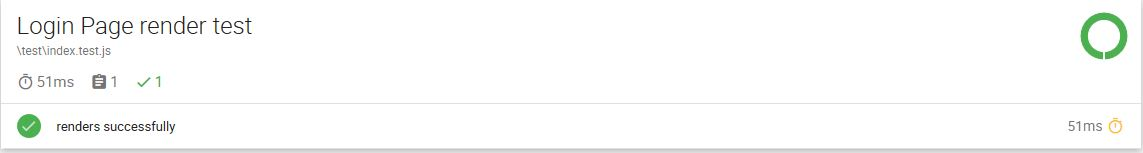
\includegraphics[width=1\linewidth]{Graphics/MochaTest1.JPG}
    			\caption{Login page render test}
    			\label{fig:loginTestRender}
	 	    \end{figure}
		
						\subsubsection{Comment}
				In Figure \ref{fig:loginTestRender} it can be seen the test passed.Therefore the login page renders and there are no errors with the login page.
			
		\subsection{Test 2}
		\subsubsection{ Explanation }
		This tests checks whether data can be sent to the login page without any errors.\linebreak
		
		\subsubsection{Test Code}
			\begin{verbatim}
			request(app)
			.get('/')
			.set('Accept', 'application/json')
			.set('Content-Type', 'application/json')
			.send({ username: 'Seonin', password: 'Seonin' })
			.expect(200)
			.end(done);
			\end{verbatim}
			
		\subsubsection{Test results}
		\begin{figure}[h]
			\centering
		    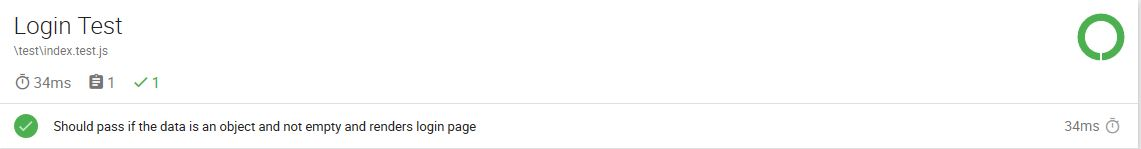
\includegraphics[width=1\linewidth]{Graphics/MochaTest2.JPG}
			\caption{Login test}
			\label{fig:loginTest}
	 	\end{figure}
		
		\subsubsection{Comment}
		Figure \ref{fig:loginTest} shows that the test passes because it can send the object to the page and the page will still render.
		
	\subsection{Test 3}
		\subsubsection{Explanation}
		This test will try to route to a page that does not exist and expect a 404 page not found error code.
		\subsubsection{Test Code}	
		\begin{verbatim}
			request(app).get('/unknown_page').expect(404, done);
		\end{verbatim}
		\subsubsection{Test results}
		\begin{figure}[h]
			\centering
		    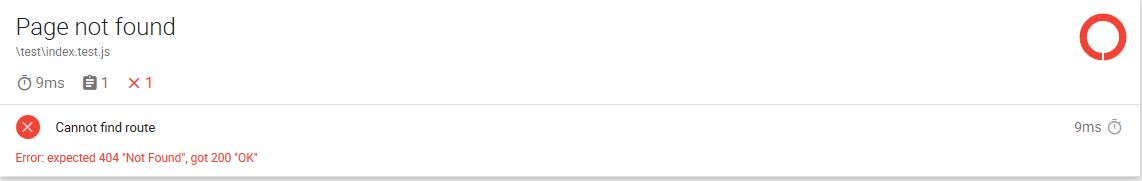
\includegraphics[width=1\linewidth]{Graphics/MochaTest3.JPG}
			\caption{Error 404/200: Page not found error with pass on routing}
			\label{fig:Error404/200}
	 	\end{figure}
		\subsubsection{Comment}
		In Figure \ref{fig:Error404/200}. This test will fail because even though the page does not exist. We put a 404  page that will display if a page is not found.Thus it gives code 200 because it routes to the error page.
	
	\subsection{Test 4}
	\subsubsection{Explanation}
		This test expects 200 status because it should route to the error page whenever there is an error 404 code.
	\subsubsection{Test Code}	
		\begin{verbatim}
		request(app).get('/unknown_page').expect(200, done);
		\end{verbatim}
	\subsubsection{Test results}
		\begin{figure}[h]
			\centering
		    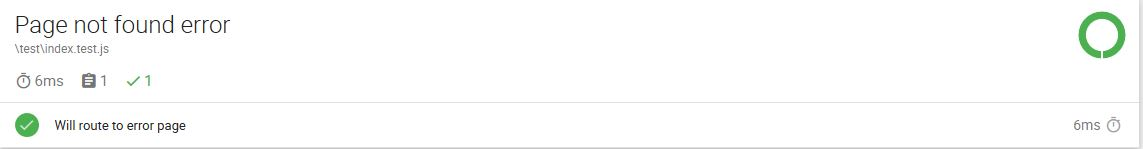
\includegraphics[width=1\linewidth]{Graphics/MochaTest4.JPG}
			\caption{Error 404: Page not found error}
			\label{fig:Error404}\fontfamily{lmss}\selectfont
	 	\end{figure}
	
	\subsubsection{Comment} 
	In Figure \ref{fig:Error404} it passes the test because a page was inserted to route to if there is an error 404 code.
	
\section{Benchmark Tests}
\subsection{Artillery testing framework}	
	For benchmark test run on Seonin David's laptop the following results were captured:
	\begin{itemize}
		\item 600 scenarios were created in 70 s
		\item All 600 scenarios returned with code 200 which means that all the requests did not produce and errors.
		\item Min latency of 6 ms
		\item Max latency of 254.8 ms
		\item Mean latency of 118.7 ms
	\end{itemize}

\subsection{Loadtest testing framework}
\begin{itemize}
	\item Target URL: \textbf{https://localhost:4000/}
	\item Time: 50s
	\item Concurrency level: 100
	\item Requests per second: 140
	\item Completed requests:  10175
\end{itemize}
\end{document}
